%Librerías a usar---------------------------------------------------------------------
\documentclass[11pt, twocolumn]{llncs}
\usepackage[spanish]{babel}
\usepackage[utf8]{inputenc}
\usepackage{multicol}
\usepackage{geometry}
\usepackage{graphicx}
\usepackage{wrapfig}
\usepackage{listings}
\usepackage{hyperref}
\usepackage{tabularx,booktabs,caption}
\newcolumntype{Z}{>{\raggedright}X}
\renewcommand\spanishtablename{Tabla}
\geometry{top=1in, left=1in, right=1in}

%Inicio del documento-----------------------------------------------------------------
\begin{document}

%Título y autores---------------------------------------------------------------------
\title{TIEMPO DE EJECUCIÓN DE UN ALGORITMO DE MATRICES CUADRADAS}
\author{
Germán Contreras  \and 
Luciano Grandi  \and
Luis Correa \and 
Rodrigo Aguirre  \\ 
 \email{\{usuario1\}\{usuario2\}\{usuario3\}\{usuario4\} @utem.cl}
}
\institute{Universidad Tecnológica Metropolitana del Estado de Chile, Santiago, Chile
}
\maketitle

%Resumen del documento----------------------------------------------------------------
\begin{abstract}
i dont know
\end{abstract}

%INTRODUCCIÓN
\section{INTRODUCCIÓN}


%CONTEXTO Y PROPÓSITO DEL EXPERIMENTO
\section{CONTEXTO Y PROPÓSITO}\label{contexto_proposito}

Un algoritmo es un conjunto de instrucciones definidas, o secuencias de pasos lógicos que permiten solucionar un problema o realizar una tarea determinada. Estos algoritmos pueden clasificarse acorde a su complejidad, ya sean sencillos o complejos. Al disponer de un algoritmo que funcione correctamente, se nos hace útil determinar ciertos criterios para cuantificar su comportamiento, o en otras palabras, su rendimiento.

Muy seguido se piensa que al hablar de algoritmos sencillos, estos no son competentes. Pero, a la hora de modelar un algoritmo, la sencillez es un componente muy interesante, dado que agiliza el estudio de su eficiencia y su mantenimiento. Cuando hablamos de rendimiento en un algoritmo, este se mide respecto a dos parámetros: el espacio de memoria y el tiempo de ejecución.

Se denomina como tiempo de ejecución de un algoritmo al rango de tiempo t en que un algoritmo comienza su proceso de ejecución hasta el término de este. Este tiempo dependerá de varios factores, tales como la calidad del código o la complejidad del mismo, y los datos de entrada.

Los datos de entrada (dependiendo del tamaño) al interactuar en un algoritmo, tendrán distintos comportamientos y tiempos de ejecución, tal como muchas funciones matemáticas que existen. Esta comparación no es trivial, dado que al saber la complejidad de una función matemática, podemos relacionarla con algún algoritmo y determinar de forma teórica su grado de dificultad. Este grado de dificultad se puede usar para determinar a qué orden de complejidad corresponde cada algoritmo, y así encontrar el que mejor se adapte al problema a solucionar.

Para tal efecto, se desarrollará un algoritmo que pueda crear y multiplicar dos matrices cuadradas de tamaño n. Una matriz es un arreglo bidimensional con un conjunto de datos, ordenados en filas ($i$) y columnas ($j$). Existen diversos tipos de matrices, como las matrices nulas, donde sus datos son solo ceros o las matrices cuadradas, las cuales tienen el mismo número de filas y columnas tal que \textit{n = i = j}.

\begin{figure}
\centering
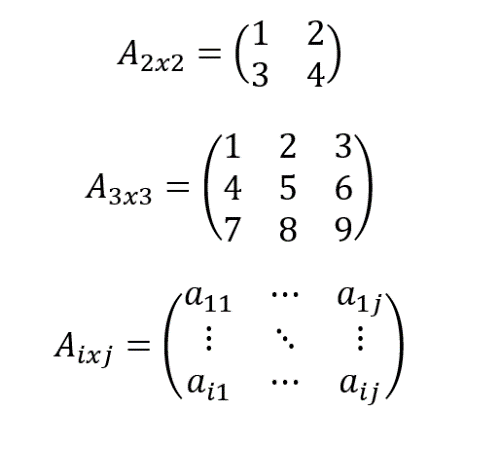
\includegraphics[width=0.3\textwidth]{matrices.png}
\caption{\label{fig:matrices}Ejemplo de matrices cuadradas.}
\end{figure}


\end{document}